

\documentclass{article}




\usepackage{graphicx}
\usepackage[large]{subfigure}

\usepackage{lipsum}
\usepackage[utf8]{inputenc}
\usepackage{csvsimple}


\usepackage{bm}
\usepackage{soul}
\usepackage{rotating}


\usepackage[shortlabels]{enumitem}


\newcounter{questioncounter}

\newenvironment{question}{% 
  \refstepcounter{questioncounter}
 \list{\thequestioncounter .}{%
 \item
   \begingroup
 }%
 \endgroup
}{\endlist}



% George: I added the following package to solve a problem in my machine about finding figures, please let me know if it does not work for you:
\usepackage{grffile}

\usepackage[utf8]{inputenc}
\usepackage[english]{babel}

\setlength{\parindent}{0.6em}
\setlength{\parskip}{0.2 em} 

\makeatletter
\renewcommand{\paragraph}{%
  \@startsection{paragraph}{4}%
  {\z@}{0.2 ex \@plus 1ex \@minus .2ex}{-1em}%
  {\normalfont\normalsize\bfseries}
}
\makeatother




\renewcommand{\baselinestretch}{1.2}


\usepackage[font=large]{caption}
% Si on veut des mini-tables des matières (utiliser minitoc-hyper 
% en conjonction avec tulhypref) :
\usepackage[english]{minitoc}
\usepackage{arydshln}
%\usepackage{comment}




%%%%%%%%%%%%%%%%%%%%%%%%%%%%%%%%%%%%%%%%%%%%%%%%%%%%%%%%%%%%%%%%%%%%%%%%%%
%Packages added by George 
\usepackage[margin=1.4 in]{geometry}
\usepackage[colorlinks=true,urlcolor=blue,linkcolor=blue,citecolor=black]{hyperref}

%\addbibresource{ReadingCourse (1).bib}

\usepackage[T1]{fontenc}  
\usepackage[utf8]{inputenc}
\usepackage{times} 
\usepackage{amsmath}
\usepackage{amsfonts}  
\usepackage{amssymb}
\usepackage{mathtools}
%\usepackage{amscd}     
%\usepackage{hyperref}   
%\usepackage[dvipsnames]{xcolor}  


\usepackage{multirow}
\usepackage{amsthm}
\usepackage{color}

\usepackage[alphabetic,y2k]{amsrefs} 
%\usepackage[all]{xy}\SelectTips{cm}{}
\usepackage{cleveref}



\usepackage{qtree}

\crefname{subsection}{subsection}{subsections}

\usepackage{stmaryrd}
%%%%%%%%%%%%%%%%%%%%%%%%%%%%%%%%%%%%%%%%%%%%%%%%%%%%%%%%%%%%%%%%%%%%%%%%%%
\usepackage{url}
\usepackage{enumitem}
\usepackage{mathrsfs}     
\usepackage[normalem]{ulem} %for sout
\usepackage{lineno}
\usepackage{mathtools}




\usepackage[parfill]{parskip}
\usepackage{bigstrut}
\usepackage{cmbright}
\renewcommand{\familydefault}{\sfdefault}
\usepackage{tikz}
\usetikzlibrary{arrows}
\usetikzlibrary{shapes.geometric}
\usetikzlibrary{shapes.multipart}
\usetikzlibrary{positioning}
\usetikzlibrary{trees}
\pgfkeys{/pgf/rectangle split parts=10}
\newlength{\MMtextNodeWidth}
\newcommand{\MMsetTextNodeWidth}[1]{%
  \settowidth{\MMtextNodeWidth}{#1}%
}



\DeclarePairedDelimiter\ceil{\lceil}{\rceil}
\DeclarePairedDelimiter\floor{\lfloor}{\rfloor}

\theoremstyle{plain}
\newtheorem{thm}{Theorem}[section]
\newtheorem{lem}[thm]{Lemma}
\newtheorem{cor}[thm]{Corollary}
\newtheorem{prop}[thm]{Proposition}
\newtheorem{conj}[thm]{Conjecture}
\newtheorem{dfn}[thm]{Definition}
\newtheorem{nota}[thm]{Notation}
\newtheorem{rem}[thm]{Remark}
\newtheorem{dfnnota}[thm]{Definition and Notation}
\newtheorem{notarem}[thm]{Definition and Remark}
\newtheorem{ex}[thm]{Example}



\newtheorem{claim}[thm]{Claim}

\newtheorem{prob}[thm]{Problem}
\newtheorem{ass}[thm]{Assumption}
\newtheorem{obs}[thm]{Observation}
\newtheorem{moti}[thm]{Motivation}
\newtheorem{cons}[thm]{Construction}
\newtheorem{setup}[thm]{Computational Setup}
\newtheorem{dfns}{Definitions}[section]
\newtheorem{axiom}[thm]{Axiom}
\newtheorem{dis}[thm]{Discussion}
\numberwithin{equation}{section}

%\numberwithin{figure}{section}



%Figure numbering, added by George 

 


\renewcommand{\labelenumi}{(\arabic{enumi})}
\renewcommand{\labelenumiii}{(\roman{enumiii})}
\renewcommand{\theenumi}{\alph{enumi}}
\renewcommand{\labelenumi}{(\theenumi)}
\renewcommand{\theenumii}{\roman{enumii}}
\renewcommand{\labelenumii}{(\theenumii)}

\usepackage{listings}
\usepackage[ ruled,vlined , titlenumbered,ruled,noend,algo2e]{algorithm2e}
\newcommand\mycommfont[1]{\large\ttfamily\textcolor{blue}{#1}}
\SetCommentSty{mycommfont}
\newsavebox{\codebox}
\newsavebox{\codeboxa}
\newsavebox{\codeboxb}
\newsavebox{\codeboxu}


%\usepackage[noend]{algorithmic}  
\usepackage{algorithm}

%semiAlgorithm environment
\makeatletter
\newcounter{algorithmbis}
\setcounter{algorithmbis}{0}
\renewcommand{\thealgorithmbis}{\arabic{algorithmbis}}
\def\algorithmbis{\@ifnextchar[{\@algorithmbisa}{\@algorithmbisb}}
\def\@algorithmbisa[#1][#2]{%
 ~\refstepcounter{algorithmbis}
  \trivlist
  \leftmargin\z@
  \itemindent\z@
  \labelsep\z@
  \item[\parbox{\textwidth}{%
    \hrule
    \hrule
    \noindent\strut\textbf{ #1 \thealgorithmbis}#2 
    \hrule
  }]\hfil\vskip0em%
}
\def\@algorithmbisb{\@algorithmbisa[]}
\def\endalgorithmbis{\hfil\vskip-1em\hrule\endtrivlist}
\makeatother

%\renewcommand{\algorithmiccomment}[1]{  $\triangleright$ #1}
%\renewcommand{\algorithmicrequire}{\textbf{Input:}}
%\renewcommand{\algorithmicensure}{\textbf{Output:} }
%\newcommand{\termin}{\hspace{-0.84 cm } \textbf{Termination Condition:}}
% End: Algorithm environment







\newcommand{\Boxx}{\rm{Box}} 

%%%%%%%%%%%%%%%%% REVIEW COLORS  %%%%%%%%%%%%%%%%%%%%%%%%%%%%%%%%%%%%%%
\usepackage{xspace}
\newcommand{\revisionNewOld}[2]{{\color{blue}#1\xspace}{\color{red}\sout{#2}\xspace}}
\newcommand{\revisionAdd}[1]{{\color{blue}#1\xspace}}
\newcommand{\revisionMargin}[1]{\textcolor{blue}{$\star$}\marginpar{\scriptsize\color{blue}
    {$\star$ #1}}}
\newcommand{\revisionMarginNoStar}[1]{\marginpar{\scriptsize\color{blue}  {#1}}}
\newcommand{\markRevCom}[2]{\marginpar{\scriptsize\color{blue}  {Reviewer~#1,
      Comment~#2}}}
\newcommand{\revisionCertified}[1]{{\color{brown}#1\xspace}}

%% SWITCH BETWEEN COMMENTED OR NOT COMMENTED VERSIONS
\newcounter{version}
\setcounter{version}{0}
\setcounter{version}{1}
% 0 means version with colors and margin comments
% 1 means version with without colors and without margin comments, that is true
% final version
\ifnum \value{version}=1
  %% REMOVE COLORS and margin comments
  \renewcommand{\revisionNewOld}[2]{{#1\xspace}}
  \renewcommand{\revisionAdd}[1]{{#1\xspace}}
  \renewcommand{\revisionMargin}[1]{}
  \renewcommand{\revisionMarginNoStar}[1]{}
  \renewcommand{\markRevCom}[2]{}
  \renewcommand{\revisionCertified}[1]{{#1\xspace}}








\newcommand*{\logeq}{\ratio\Leftrightarrow}
\newcommand{\spec}{\operatorname{spec}}
\newcommand{\Gr}{\operatorname{Gr}}
\newcommand{\Emb}{\operatorname{Emb}}


%%%%%%%%%%%%%%%%% Comments %%%%%%%%%%%%%%%%%%%%%%%%%%%%%%%%%%%%%%
% One way to insert comments
\newcommand{\george}[1]{\textcolor{brown}{\textsc{George: } {\sf #1}}}
\newcommand{\gk}[2]{{\color{blue}$\star$}\marginpar{\tiny\color{blue} George: #1\space}}
\newcommand{\gkr}[2]{{\color{red}$\star$}\marginpar{\tiny\color{red} George: #1\space}}
\newcommand{\MP}[1]{\textcolor{cyan}{\textsc{Marc: } {\sf #1}}}
\newcommand{\GM}[1]{\marginpar{\tiny\textcolor{BrickRed}{\textsc{G: }
{#1}}}}
\newcommand{\SL}[2]{{\textcolor{Red} {#1}} \sout{\textcolor{green}{#2}}}
\newcommand{\SLa}[1]{\textcolor{Red} {#1}}
\newcommand{\SLr}[1]{\sout{\textcolor{green}{#1}}}
%% Without comments:
%\renewcommand{\SL}[2]{{\textcolor{Red} {#1}}}
%\renewcommand{\SLa}[1]{\textcolor{Red} {#1}}
%\renewcommand{\SLr}[1]{}
% another way
\newcommand{\ste}[1]{\par\noindent\textcolor{blue}{\small Stephan: #1}}
\newcommand{\marc}[1]{\textcolor{cyan}{$\star$}\marginpar{\textcolor{cyan}{ \tiny
      Marc: #1}}}

%\usepackage{easyReview}
%\usepackage{authblk}


%MARC

\newcommand {\R}{\mathbb R}
\newcommand {\Q}{\mathbb Q}
\newcommand {\C}{\mathbb C}
\newcommand {\Z}{\mathbb Z}
\newcommand {\N}{\mathbb N}
\newcommand {\Cn}{\mathfrak{C}}
\newcommand {\Cnb}{\overline{\Cn}}
\newcommand {\LL}{\mathfrak{L}}
\newcommand {\Lc}{\LL_{\rm c}}
\newcommand {\Lcp}{\Lc^{\prime}}
\newcommand {\Ln}{\LL_{\rm n}}
\newcommand {\Lnp}{\Ln^{\prime}}
\newcommand {\Lh}{\widehat{\LL}}
\newcommand {\Lnh}{\Lh_{\rm n}}
\newcommand {\Lch}{\Lh_{\rm c}}
\newcommand {\Ball}{\mathrm{Ball}}
\newcommand {\codim}{\mathrm{codim}}
\newcommand{\Ub}{\overline{\mathfrak{U}}}

\newcommand{\Pt}{\widetilde{P}}
\newcommand{\calA}{\mathcal{A}}
\newcommand{\rank}{\operatorname{rank}}
\newcommand{\ord}{\operatorname{ord}}
\newcommand{\Bbox}{\mathfrak{B}}
\renewcommand{\le}{\leqslant}
\renewcommand{\leq}{\leqslant}
\renewcommand{\ge}{\geqslant}
\renewcommand{\geq}{\geqslant}
\newcommand{\mult}{\operatorname{mult}}
%%%%%%%%%%%%%%%%%%%%%%%%%%%%%%%%%%%%%%%%%%%%%%%%%%%%%%%%%%%%%%%%%%%%%%%%%%%%%%%%

%%%%For embadding codes 
\definecolor{codegreen}{rgb}{0,0.6,0}
\definecolor{codegray}{rgb}{0.5,0.5,0.5}
\definecolor{codepurple}{rgb}{0.58,0,0.82}
\definecolor{backcolour}{rgb}{0.95,0.95,0.92}

\lstdefinestyle{mystyle}{
    backgroundcolor=\color{backcolour},   
    commentstyle=\color{codegreen},
    keywordstyle=\color{magenta},
    numberstyle=\tiny\color{codegray},
    stringstyle=\color{codepurple},
    basicstyle=\ttfamily\footnotesize,
    breakatwhitespace=false,         
    breaklines=false,                 
    captionpos=b,                    
    keepspaces=true,                 
    numbers=left,                    
    numbersep=5pt,                  
    showspaces=false,                
    showstringspaces=false,
    showtabs=false,                  
    tabsize=1
}

\lstset{style=mystyle}

%%%%%%%%%%%%%%%%%%%%%%%%%%%%%%%%%%%%%%%%%%%%%%%%%%%%%%%
%For controling the margin locally 
\newenvironment{changemargin}[2]{%
\begin{list}{}{%
\setlength{\topsep}{0pt}%
\setlength{\leftmargin}{#1}%
\setlength{\rightmargin}{#2}%
\setlength{\listparindent}{\parindent}%
\setlength{\itemindent}{\parindent}%
\setlength{\parsep}{\parskip}%
}%
\item[]}{\end{list}}
%%%%%%%%%%%%%%%%%%%%%%%%%%%%%%%%%%%%%%%%%%%%%%%%%%%%%%%%%%%%%%%%%%%%%%%%%%%%%%%%





\begin{document}














\section{High-level rules of translation }
  


This section is dedicated to describe the rules of the translator we define. Based on these rules.  

\subsection{Translator input}
The input is a TLA+ Spec that has the following properties. 


\subsubsection{Proc}\label{Proc} This constant is a set of integers and strings which  is used to declare the processes identifiers. The user is supposed to define it as a part of the input.  

\subsubsection{TypeOK} \label{TypeOK} As mentioned before, the TLA+ Spec is supposed to contain an invariant \emph{TypeOK}.  This predicate is required to obtain the types of variables. In Listing \eqref{TypeOkcodes}, the objects $Set\_1 \dots Set\_n$ are sets of integers boolean or function sets. For the last case, $Set\_i$ is of the form $[ Proc\_Subset \text{   -->  }  Target_i]$ where $Proc\_Subset$ is a subset of $Proc$ and $Target_i$ is a set of integers, boolean or strings. 
 Notice that the formula $xi=value\_i$ is equivalent to $xi \in Set\_i$ with $Set\_i$ is a singleton. Hence, we allow $xi=value\_i$ syntactically \footnote{Note that for the case of functions, we have the form $xi=  [Obj \text{   }\backslash in \text{   } Proc\_Subset \text{   |-->  }  \text{Expression}(Obj)] $ }.


\begin{lstlisting}[language=Python,caption={The explicit form of the predicate \emph{TypeOK}.}, label={TypeOkcodes}] 
VARIABLES x1,.., xn

TypeOK == 
          /\ x1 \in Set_1
          ....
          ....
          /\ xn \in Set_n
 
\end{lstlisting}


\subsubsection{Structure} \label{Structure}
We are going to assume that the TLA+ Spec has a simple structure. In particular,
 no labeled predicates are used as sub-expressions of (resp. next-) state relations or invariants. If any,
 we simply expand all expressions to get the following: 


\begin{lstlisting}[frame=single]
CONSTANTS c1, .. , cm


VARIABLES x1,.., xn

TypeOK == /\ x1 \in Set_1
          ....
          ....
          /\ xn \in Set_n

Invariants == (* Defining the invariants of the Spec *)           

(* I_i is a state predicate that determines the initial state of x_i *)

Init == /\ I_1    
        /\ I_2 
        .....
        .....
        /\ I_n 

(* N_i is a next-state relation (more details are below *)

Next == \/  N1 
        \/  N2 
            ...
            ...
        \/  N_k 

Spec == Init \/ []Next_<<x1, .. xn>>        
\end{lstlisting}

 We are going to  give a more precise form later on.


\subsection{Predicate $\&$ Quantified logic} \label{Sec:Pred-Quant}

We discuss here the translation of state predicates, i.e., boolean-value expressions containing variables and constants that are not  next-state relations (no primed variables).

We consider the following cases: 

\subsubsection{Simple date types} \label{SimType}

 For a variable $x$ of a simple data type (integer, boolean or string) 
\begin{enumerate} 

\item The simple (sub-)expression \emph{$x=value$}, where $x$ is a variable and  \emph{$value$} is an integer or a boolean constant. In this case, the translation is simple and straightforward.  

\item  For  the (sub-)expression \emph{$x=value$}, where \emph{$value$} is a string, a Cubicle abstract type  is defined that encodes all values of string-type variables. To compute the values, we recognize two cases: 
\begin{enumerate}
\item If the TypeOk invariant states that  $x$ takes values on a finite set of strings, that is, \emph{$x \in StringSet_x$}, then we are done with this case.



\item Otherwise, we scan the whole TLA-spec looking for (sub)expressions of the form \emph{$x=value$} or \emph{$x'=value$} computing a set \emph{$StringSet_x$}.

  \end{enumerate}


After computing StringSet of all string-type variables, we define $\operatorname{String\_values}=\{S1,\dots, Sk\}$ that is the union of all \emph{$StringSet_x$}. In the Cubicle spec, we define an abstract type \emph{$String\_type$} and \emph{$x\_i$} for each string-type variable as follows: 

\begin{lstlisting}[language=Java]
String_type = S1 | S2 | ... | Sk
var x : String_type

\end{lstlisting}
After that, every (sub-)expression of the form \emph{$x=Si$} is translated to 
$$\emph{x= Si;}$$ 


\end{enumerate}



\subsubsection{Complex date types}
We restrict our selves to the following cases: 

\begin{enumerate} 
\item  For  the (sub-)expression \emph{$x=Value$}, where \emph{$Value$} of the form:

$$ [c1 ... ck \text{ }\backslash in \text{ } Proc\_Subset \text{ }  \text{  |-->  } Value_{c1,\dots,ck} ],$$
 where $Value_{c1,\dots,ck}$ is an integer, a boolean or a string value. \emph{$x=Value$} is translated to: 
 $$ x(z1 ... zk) = Translation(Value_{c1,\dots,ck})  $$
 where $Translation(Value_{c1,\dots,ck})$ is computed as in Sec \ref{SimType}.

\item  For  the (sub-)expressions \emph{$x=Value$}, \emph{$x'=Value$} where \emph{$Value$} of the form:

$$ [Value_{old}  \text{ } EXCEPT \text{ } ![c1] =e1, ..., ![ck] =ek \text{ }  ],$$
 where $e1,\dots,ek$ are integers,  booleans or strings values and $Value_{old}$ is a constant function of the same type of the one defined in (a), then the expression \emph{$x=Value$} is translated to: 

\begin{align*}
x(z) &= case\\
& | \text{ } z = c1 : e1 \\
& | \text{ } z = c2 : e2 \\
&  ... ... \\
& |\text{ }  z = ck : ek \\
& | \_ : Value_{old};
\end{align*}


%\begin{align*}

% x(z1 ... zk) = case \text{ } | \text{ } z1 = e1  \\
% \text{ }  ... \text{ } \\
%  zk=ek\text{ }  : Value_{c1,\dots,ck} 
%  \text{ } | \_ : Value_{old}[z1 ... zk] 
%  \end{align*}
 
\end{enumerate} 


\subsubsection{Locating  the translation of state predicates}

Depending on the position of the TLA-expressions,  we its the translation: 

\begin{enumerate}
\item  (sub-)expressions appearing in the TLA++ initial state are translated to  predicates  in the initial Cubicle one.   
\item The translation of (sub-)expressions of invariant negations are located in the unsafe predicate in the Cubicle Spec.  
\item The (sub-)expressions in the next state are translated to the \emph{requesters} part of a Cubicle \emph{transition}. 


\end{enumerate}




\subsection{Initial state} 
Suppose that the spec has the variables $x1, \dots, xn$ of types determined by the invariant TypeOK as described in Sec~\ref{TypeOK}.  We consider the following form of the initial state:

\begin{lstlisting}
Init == /\ x1= Value_1  
        /\ x2= Value_2  
        .....
        .....
        /\  xn= Value_n   
\end{lstlisting}
\george{The blue parts of the rest concern the multi-dimensional case. I keep them, however, I ignore  them in the algorithm and the grammar for the moment.  }
\color{blue}
We are going to describe in details how to translate the initial state depending on the "shape" of $Value_i$: Let $h$ be the maximal dimension of the tuple variables, i.e., $h=\max\{dim(xi)\mid 1\leq i \leq n\}$\footnote{By dimension we mean the minimum number of indexes needed to parametrize $xi$.} The translation of \emph{Init}  is parametrized by $h$ variables, that is, the Cubicle intial state takes the form 
\begin{lstlisting}[language=java]
init (z1 ... zh)   { Translation(x1= Value_1) 
                   &&  Translation(x2= Value_2) 
                    ... 
                   && Translation(xn= Value_n)  }
\end{lstlisting} \color{black}
  Now we determine (when possible) more explicitly  how to compute  $\emph{Trans(xi= Value\_i)}$. We consider the following cases: 





\begin{enumerate}
\item  \emph{$Value\_i$} is an integer or boolean value, then the translation is straightforward. For  the case where \emph{$Value\_i$} is a string, an abstract type is already defined with  \emph{$Value\_i$} is  one of its values (Section~\ref{Sec:Pred-Quant}). 
\item  \color{blue} $Value\_i= [Obj \text{  }\backslash in \text{  }  Proc\_Subset \text{  |--> } Target_i]$, where  $Target_i$ is a constant function (not necessarily declared as a constant\footnote{For example, $Value\_i= [Obj \text{  }\backslash in \text{  }  Proc\_Subset \text{  |--> } k]$ with $k$ is an integer.}) with the domain $Proc\_Subset$. Then, $xi=Value\_i$  is translated to 

$xi[Xi]=Target_i[X_i]$, where $X_i = \{z1 \dots zi\} $ and $i=dim(Proc\_Subset)$. A condition to check is $dim(Proc\_Subset)=dim(xi)$. The type of $Target_i[X_i]$ is integer, boolean or string. Again, for the case where $Target_i[X_i]$ is a string, an abstract type is already defined with $Target_i[X_i]$ is  one of its values (Sec~\ref{Sec:Pred-Quant}).\color{black} 


\item For a constant $Proc\_Subset$,  $\emph{case\_1, \dots, case\_k}$ are state predicates, and $\emph{Value\_i1, \dots, Value\_ik}$ are state functions of integer, boolean or string type,  if $xi$ is initialized as follows: 
\begin{lstlisting}[language=Python]
xi = [self \in Proc\_Subset |-> CASE case_1 -> Value_i1
                 [] case_2 -> Value_i2
                      ....
                 [] case_k -> Value_ik
\end{lstlisting} 
then the translation is of the form:

\begin{lstlisting}[language=java ]
(x_1[X1] =  Trans(Value_i1)  &&  Trans(case_1) )
|| (x_2[X2] =  Trans(Value_i2)  &&  Trans(case_2))    
   ...
   ...  
|| (x_k[Xk] =  Trans(Value_ik)  &&  Trans(case_k)) 
\end{lstlisting}
See Sec~\ref{Sec:Pred-Quant} for the translation  and the restrictions on the  state predicates $\emph{case\_1, \dots, case\_k}$ and state functions.

\item As a special case $xi  \text{ }\backslash in \text{ } \{e1, \dots, ek\}$, where $ei$ is of type integer, boolean or string. Then,  the translation is 
\begin{lstlisting}[language=java]
   x_i =  e1   
   || x_i =e2    
   ...
   ...  
   || x_i=ek  
\end{lstlisting}





\end{enumerate}


 


\subsection{Next state} 

Assume that the Next predicate is of the form: 

\begin{lstlisting}[language=Python]
Next == \/  N1 
        \/  N2 
            ...
            ...
        \/  N_k 
\end{lstlisting}

where $Ni$ is one of the following: 
\begin{enumerate}
\item $Ni= P_p /\backslash (xi'=P_n)$, with $P_n$ and $P_p$ are state function and state predicate respectively.  Then, the translation is of the form: 
\begin{lstlisting}[language=Java]
transition Ni() 
requires {  Trans(P_p) }
{ xi:= Trans(P_n);}

\end{lstlisting}

$Trans(P_p)$  and $P_n$  can be computed as in Sec~\ref{Sec:Pred-Quant}




\item $Ni=$ \emph{$\backslash E \text{ } \text{ }z \text{ } \backslash in \text{ } Proc\_Subset: P_p(z) /\backslash (xi'=P_n(z))$,} 
 with $P_n$ and $P_p$ are state function and state predicate respectively. Then, the translation (with the abuse of notation for $z$) is of the form: \footnote{Clearly, the sub-formula $(xi'=P_n(z))$ in this case can be generalized to the multi-variable one. }
\begin{lstlisting}[language=Java]
transition Ni(z) 
requires {  Trans(P_p(z)) }
{ Trans(xi = P_n(z))}
\end{lstlisting}




\item \george{The idea of Case(c) is a remark that you mentioned on a meeting. I hope that I understood it collectedly. I still do not considered it in the Algo, until you confirm it.  }Suppose we have that: 
\begin{lstlisting}[language=Java] 
Ni== \E z \in Proc : (\A y \in Proc : x[y]'= Value_y)
\end{lstlisting}
where $Value_y$ is an integer, boolean or string.  Then the translation of $Ni$ is computed as in the case: 
\begin{lstlisting}[language=Java] 
Ni== x'=[y \in  |-> Value_y ]
\end{lstlisting}

\color{blue}
\item A generalization of (b) is the multivariable case $z1, \dots, zk$ can be analogously done. 
\color{black}

\end{enumerate}





\section{Grammar of the fragment } \label{Grammar}
Since the illustration of codes below is still too bad, I suggest to read the grammar details in $"TlaplusToCubicle/grammer/Trans\_Input\_Gram.tla"$ until I find a way to improve it as a Latex environment. 

\begin{lstlisting}
------------------------------ MODULE FragGram ------------------------------
( * We use  BNFGrammars https://github.com/tlaplus/Examples/blob/master/specifications/SpecifyingSystems/Syntax/BNFGrammars.tla * ) 



Spec == Init 
        & tok("\/") 
        & tok("[][") 
        & Next 
        & tok("]_") 
        & VARIABLES


VARIABLES == tok("<<")  
             & ( Identifier 
             & (tok(",") & Identifier)^* ) 
             & tok(">>")


(* ############################################################################################ *)
(* ########### Defining the Init part ######################################################### *)
(* ############################################################################################ *)

Init == (tok('/\') & Simple_Propositional_Exp)^+
Simple_Propositional_Exp ==  (Identifier & tok("=") & VALUE)   
                             |  (Identifier & tok("\in") & Finite_Set)

Finite_Set == tok('{') 
                & Value 
                & (tok(",") & Value)^*
                &  tok('}') 
              | Numeral^+ & tok("..") & Numeral^+
              | Numeral^+ & tok("..") &  Identifier
              | Identifier & tok("..") &  Numeral^+
              | Identifier & tok("..") &  Identifier  
 

VALUE == Identifier (* I have a constant in mind *) 
         | Numeral^+ 
         | Numeral^+ & tok(".") & Numeral^*
         | STRING 
         | Boolean   
         | Function
         | Identifier  & tok("[") & (TERM) & tok("]")
         | Identifier  & tok("(") & (TERM) & tok(")")
          

Function == tok('[')     
                & Identifier 
                & tok(' \in ') 
                & Identifier  (* I have a subset of Proc in mind*)
                & tok('|->') 
                & TERM
                & tok(']') 


(* In the following, Tok(P) means that the set of all terms of the form P  *)
STRING == Tok (tok(" " ") & NameChar^* & tok(" " ") )  \ ReservedWords (* The same ReservedWords defined in TLAPlusGrammar.tla *)

Boolean == tok("True") | tok("False")

Identifier == Name \ ReservedWords
Name == Tok((NameChar^* & Letter & NameChar^*))
NameChar  == Letter \cup Numeral \cup {"_"}  
Letter == OneOf("abcdefghijklmnopqrstuvwxyzABCDEFGHIJKLMNOPQRSTUVWXYZ")
Numeral   == OneOf("0123456789") 


(* ############################################################################################ *)
(* ########### Defining the Next part ######################################################### *)
(* ############################################################################################ *)

Next ==  (tok('\/') & Next_State_Exp)^+


Next_State_Exp ==    (tok('/\') & Predicate)^*
                     & (tok('/\') & Primed_Exp)^+

(* ################################################ *)
(* ########### Defining Predicate ################# *)
(* ################################################ *)
 
 Predicate ==  Propositional_Exp         
               |  tok("(") 
                  & (tok('\E') | tok('\A'))  
                  & Identifier (* For the moment, let us stay in the one-variable case *)
                  & tok("\in")
                  & Identifier  (* I have a subset of Proc in mind *)
                  & tok(' : ') 
                  & Predicate
                  & tok(")")
                  
Propositional_Exp ==  Simple_Propositional_Exp 
                      | tok("(") & TERM & OPERATOR & TERM & tok(")")
                      | tok('~') & tok("(")   & Propositional_Exp & tok(")")
                      | tok("(")   
                        & Propositional_Exp  
                        & Logical_Junctions
                        & Propositional_Exp
                        & tok(")")


OPERATOR == tok("=")  |  tok("#") | tok("~=") | tok("<")  | tok("<=")


Logical_Junctions == tok("/\") | tok("\/")


TERM == VALUE | Open_Prpos



Open_Prpos == Identifier    
             | Identifier  & tok("[") & TERM & tok("]")
             | Identifier  & tok("(") & TERM & tok(")")
             (* generalize it more? *)
             
(* ################################################ *)
(* ########### Defining Primed_Exp ################ *)
(* ################################################ *)


Primed_Exp ==   Identifier 
                & tok(' ' ') 
                & tok("=")  
                & (TERM | Function_Except)
             
Function_Except == tok("[") 
                   &  Identifier  
                   & tok("EXCEPT") 
                   & ( tok('![') &  Identifier & tok(']=') & TERM 
                     & (tok('![') &  Identifier & tok(']=') & TERM )^+ ) 
                   & tok("]")
\end{lstlisting}





\section{Translating algorithm} 

\begin{lrbox}{\codebox}
   \begin{lstlisting}[language=java]
init (z)   { Translation(x1= Value_1) 
             &&  Translation(x2= Value_2) 
               ... 
             && Translation(xn= Value_n)}
\end{lstlisting}
\end{lrbox}


\begin{lrbox}{\codeboxa}
   \begin{lstlisting}[language=java]
transition Ti (z)  
requires {     
            Translation(Predicate_i)   }
          {
          Translation(xj1=Valuej1);
            ... 
            ...
          Translation(xj1=Valuejh);
          }  
\end{lstlisting}
\end{lrbox}



\begin{lrbox}{\codeboxb}
   \begin{lstlisting}[language=java]
x(z) = case |  z = c : e 
            |_ : Value_{old}[z]

\end{lstlisting}
\end{lrbox}




\begin{lrbox}{\codeboxu}
   \begin{lstlisting}[language=java]
unsafe (z) = Translating(~ Invar_1) 
            || Translating(~ Invar_2)
               ...
               ...
            ||  Translating(~ Invar_s)

\end{lstlisting}
\end{lrbox}

\begin{algorithm}[H]
\SetAlgoLined
\SetKwInOut{Input}{Input}
\SetKwInOut{Output}{Output}
    
\Input{A TLA++ Spec based on the grammar of Section~\ref{Grammar} with \emph{TypeOk}  (Section~\ref{TypeOK} invariant and constant \emph{Proc} (Section~\ref{Proc}).}
\Output{A Cubicle Spec that is equivalent to the one in the input. }
\setcounter{AlgoLine}{0}
\SetKwFunction{prepa}{prepa} \SetKwFunction{algo}{algo}\SetKwFunction{proc}{proc}

  \SetKwProg{inari}{Data-Type Preparation}{}{}
         \inari{}{ 
                    \nl Simply structure as mentioned in Sec~\ref{Structure}  

                    \nl $\operatorname{String\_values}:= \{\}$

                   \nl \For{all variables $x_i$} {
                       \nl Compute all $Type(x_i)$ from Invariant TypeOk \

                    \nl   \uIf(){$Type(x_i) =String $}

                    \nl{ Find all possible values of $x_i$ and add them to  $\operatorname{String\_values}$. This can be obtained from TypeOk invariant or scanning all possible values of $x_i$ as described in Sec~\ref{SimType}.  }
                                               }
                 } 
  \SetKwProg{myalg}{Translating Init}{}{}
  \myalg{}{
  \tcp{Recall that Init == $ \bigwedge\limits_{i=1}^n (x_i = Value_i \text{ or } x_i \in \operatorname{Finite\_set}_i ) $  }
  \For{$i=1$ \KwTo $n$}
      {   
         \uIf(){$Type(Value) \in \Z  \cup \{ True, False\} $}{
                            \nl $Translation(x_i = Value_i) := x_i = Value_i$ \;
                           }

         \uElseIf{ $Value_i = "Text_i"$ }{
                                  \nl $Translation(x_i = Value_i) := x_i = Text_i$ \;}  
         \tcp{In the following, $Proc\_Subset$ is a subset of $Proc$}
         \uElseIf{ $Value_i = [z \text{ } \backslash  in \text{ } Proc\_Subset \text{ } |-> \text{ } Value_{i,z} ] \text{ } $ }
         {
         \tcp{with $Type(Value_{i,z}) \in \{Integer, Boolean, String\}$}
                                  \nl $Translation(x_i = Value_i) := x_i(z) =  Value_{i,z}$ \;

                                  \george{Will consider multi-dim functions later}
                                } 

       \uElseIf{ $x_i \in \operatorname{Finite\_set}_i:=\{e_1,\dots, e_p\} $ }
         {
         \tcp{s.th any element $Type(e_i)$ is in $\{Integer, Boolean, String\}$}
                                  \nl $$ Translation(x_i \text{ } \backslash in \text{ } \operatorname{Finite\_set}_i) := x_i = e\_1 || \dots || x_i=e\_p$$ \;

                                } 

       }
  \nl The translation of Init is: \   
  \usebox{\codebox}}{}
  \setcounter{AlgoLine}{0}
  \SetKwBlock{myproc}{myproc}{}
 
  \SetKwProg{myproc}{Translating Next}{}{}
  \myproc{}{ 
             \tcp{Recall that Next == $ \bigvee\limits_{i=1}^k (Predicate_i \bigwedge (x_i^{\prime}=Value_i)) $  }
             \nl  \For{$i=1$ \KwTo $k$}
                                    {  
                                    \nl Define a Cubicle-transition $T_i$  as follows:     \;
                                     
                                      {}

     }{}  
            }  
            \end{algorithm}

                                                
                                                                        

                                                                                
                                   

%\SetNlSty{texttt}{(}{)}
\SetNlSty{texttt}{(}{)}
\SetKwBlock{transition}{Defining Transition $T_i$}{transition}{}
\begin{algorithm}  
\SetKwProg{inaria}{Translating invariant}{}{}            
  \LinesNumbered
\setcounter{AlgoLine}{12}
% This is to restore vline mode if you did not take the package as \usepackage[linesnumbered,ruled,vlined]{algorithm2e}
  \SetAlgoVlined
    \SetAlgoVlined
%This is to hide Begin keyword
\transition{
                                      \nl Compute $Translation(Predicate_i)$ as in Section~\ref{Sec:Pred-Quant} and place it in $T_i$ "requires"-part\;

                                      

                                     \nl  \uIf(){$\texttt{Type}(Value_i) \in \{Integer, Boolean\} $}{
                                          \nl $Translation(x_i^{\prime} = Value_i) := (x_i := Value_i)$ \;
                                                                                     } \;
                                       
                                                                     
\uElseIf{ $Value_i = "Text_i"$ }{
                                           \nl $Translation(x_i = Value_i) := (x_i =: Text_i$) \;}

\uElseIf(){ $[Value_{old}  \text{ } EXCEPT \text{ } ![c] =e  \text{ } ]$ }
{ \nl \usebox{\codeboxb}\;}

\SetKwBlock{myproc}{}{end}   

    }
              \nl The translation of Next is:\ 

              \nl \usebox{\codeboxa};
  

\inaria{}{
\tcp{Recall that $Invar\_k ==  \backslash E \text{ } Obj \text{ } \backslash  in \text{ } Proc : P(Obj), $  }
\tcp{where $P$ is a proposition respecting the rules of Sec~\ref{Sec:Pred-Quant} }
\george{next step: considering invariants with $Obj1,Obj2 in Proc$}


\nl Translate the negation of each invariant  $Invar_1, \dots, Invar_s$ as in Section~\ref{Sec:Pred-Quant}   ;\


\nl Define unsafe (z) as: 
\usebox{\codeboxu}

}

 \Return  Cubicle-spec with the computed \emph{unsafe (z), Init (z)}  and \emph{$T_1(z),\dots,T_{k}(z)$}.
 \caption{TLA++ - Cubicle Translator}
\end{algorithm}


\iffalse  

\large
\MMsetTextNodeWidth{99}

\george{Illustration of the grammar of the file $Trans\_Input\_Gram.tla$. Not ready yet}



   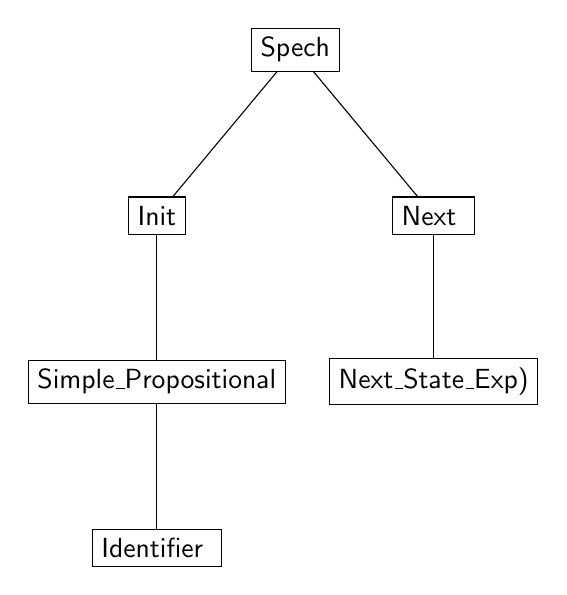
\begin{tikzpicture}
      [sibling distance=10em,level distance=6em,
      every node/.style={shape=rectangle,draw,align=center}]
\node{Spech}
   child{node{Init}
      child{node{Simple$\_$Propositional}
        child{node{Identifier }}}}
   child{node{Next }
      child{node{Next$\_$State$\_$Exp)}}};


   \end{tikzpicture}

\fi   



\iffalse    




\color{red} George: The rest is still not ready : 
We consider the following TLA+ Spec which we want to translate.

\begin{lstlisting}[language=Python]
CONSTANTS c1, .. , cm

ASSUME   (* declaring the the constants values, e.g., c1= 5   *)  

VARIABLES x1,.., xn

TypeOK == 
          /\ x1 \in Set_1
          ....
          ....
          /\ xn \in Set_n

Invariants == (* Defining the invariants of the Spec *)           

(* I_i is a state predicate that determines the initial state of x_i *)

Init == /\ I_1    
        /\ I_2 
        .....
        .....
        /\ I_n 

(* N_i is a next-state relation (more details are below *)

Next == \/  N1 
        \/  N2 
            ...
            ...
        \/  N_k 

Spec == Init \/ []Next_<<x1, .. xn>>        
\end{lstlisting}
 

\section*{Rules of translation}

 \bibliographystyle{unsrt}
\bibliography{bibl}






\subsection{CONSTANTS} Each TLA-constant $ci$ is  translated in a straightforward  way  by:  
   
\begin{lstlisting}[language=Java]
const ci : Type(ci) 
\end{lstlisting}

\emph{$Type(ci)$} is obtained by "ASSUME" expression. If \emph{$Type(ci)$} is Int, BOOLEAN or a tuple of integer or boolean values, then its translation is int,  bool or array respectively.\footnote{Indeed, it is possible to define multi-dimensional tuples in Cubicle language as done in Example \emph{$distrib\_channels.cub$} which can be found in "Examples" folder} \george{So far, the other TLA++ data types are still not considered in this translator.  }  

\ste{Should clarify what Type(ci) can be. Int, Boolean, functions, records? And
  probably we want to handle the constant representing processes in a special
  way, mapping it to the type proc of Cubicle.}

\george{I am not sure how to recognize such a constant... Do you think we ask the user to declare that a constant represents processes?  }


\subsection*{TypeOK} \george{This predicate is required to obtain the types of variables. The objects $S\_1 \dots S\_n$ are sets of integers booleans or arrays (of integers or booleans).  } 




\subsection*{VARIABLES} For every variable $xi$, the type  \emph{$Type(xi)$} is obtained from the predicate \emph{$TypeOK$}. If \emph{$Type(xi)$} is Int, BOOLEAN, then the translation is: 

\begin{lstlisting}[language=Java]
var xi : Type(xi) 
\end{lstlisting}

If $xi$ is a tuple, then the translation is 

\ste{More precisely, xi is not a tuple but you retrieve that information from
  the type that is declared for the variable. Should clarify what kinds of sets
  are allowed in the TypeOK predicate.}

\begin{lstlisting}[language=Java]
array xi : Type(xi) 
\end{lstlisting}


\ste{Again, the exact form of the initializations in the subset of TLA+ that we
  are prepared to handle will have to be determined.}

\george{Please see my last answer below.}

\subsection*{The next-state relation} 
Assuming the existence and feasibility of \emph{$Translation(N\_i)$}, we consider several cases:


\begin{enumerate}

\item If  $N\_i$ is defined as:

\begin{lstlisting}[language=Python]
N_i == S1(x1,..,xb) /\ S2(x1,..,xb,x1',..,xb')
\end{lstlisting}
, that is, $N\_i$ has no quantifier. Then the translation of  $N\_i$ is: 


\begin{lstlisting}[language=Java]
transition N_i 

requires {  Translation(S1) }
{ Translation(S2(x1,..,xb,x1',..,xb') }

\end{lstlisting}







\ste{I presume that x1,\dots,xb are the variables? Here too we will have to fix
  the syntactic form of actions (S1 and S2 parts) that will be allowed, and then
  define the translation function accordingly. For example, do we treat
  conjunction, disjunction, conditionals, let expressions etc.
  One detail is that the TLA+ action will contain UNCHANGED predicates (or
  conjuncts xi' = xi) that will be ignored by Cubicle.}

  \george{Please see my last answer below.  }

\item If  $N\_i$ is defined as:

\begin{lstlisting}[language=Python]
N_i == \E y1 ... yb : S1(y1,..,yb) /\ S2(y1,..,yb,y1',..,yb')
\end{lstlisting}

where $S1(y1,..,yb)$  and $S2(y1,..,yb,y1',..,yb')$  are a state predicate and a next-state relation respectively, i.e., $S1$ describes the preconditioning and $S2$ defined the probed variables. Then  $N\_i$ is translated to: 

\begin{lstlisting}[language=Java]
transition N_i (y1 ... yb) 

requires {  Translation(S1) }
{ Translation(S2(y1,..,yb,y1,..,yb)) }

\end{lstlisting}

\ste{In fact, the S1 and S2 parts contain the variables xi as above as well as
  the parameters yj, but the latter only unprimed.}
  \george{To be discussed}

\item If  $N\_i$ is defined as:
\begin{lstlisting}[language=Python]
N_i == \A y . N_i' 
\end{lstlisting}
where $N\_i' $ is as $N\_i$  in (a) or (b), then the translation is 

\color{red} George: Still investigating \color{black}

\ste{Do you have a concrete example of such an action in a specification?}
\george{No,  I am very confused about the necessity and feasibility of this part. That is why it is still under progress. }
\end{enumerate}

\ste{I have the feeling that the overall shape of the translation that you
  describe applies to the disjuncts of the next-state relation, but a TLA+
  specification may contain other definitions as well (that may be building
  blocks for defining the actions that make up Next). It seems to me that we
  need to proceed top-down starting from the initial and next-state predicates.
  What these are can be identified by a ``configuration'' file as used for TLC.}

  \george{In fact, I agree that the current text considers only the shape you mentioned. However, do not you think that this is how to start from a high level. This is why I assume the existence and feasibility of \emph{$Translation(I\_i)$} and \emph{$Translation(N\_i)$}. In my plan, it is expected that I do not have an explicit form of $N\_i$ and $I\_i$. On the other hand, once I have a "good" global description of the rules of translation, the next step is to go a level lower which is where I expect to get a better idea about subset of TLA+ that can be translated to Cubicle. Do you agree?. }




\fi
\end{document}

